%\section{Compactness for Sets of Regular Patterns}
\subsection{Compactness}\label{subsec:compactness}

In this section, we define the compactness of sets of regular patterns, formally.
Then, if $\sharp\Sigma \ge 2k-1$ holds, 
we show that 
$\RPat^{k}$ has compactness with respect to the containment.

\begin{dfn}\label{def:compactness}
Let $\mathcal{C}$ be a subset of $\RPatplus$. 
For any regular pattern $p \in \RPat$ and any set $Q \in \mathcal{C}$,
the set $\mathcal{C}$ said to have {\it compactness with respect to containment}
if there exists a regular pattern $q \in Q$ such that $L(p) \subseteq L(q)$ holds if $L(p) \subseteq L(Q)$ holds.
\end{dfn}

Let $D \subset \RPat$ with $\sharp D = 2$ or $3$, and let $p,q$ be regular patterns in $\RPat$.
In the following subsections (Subsecs.~\ref{subsec:d2}--\ref{subsec:d3c}), we provide the conditions on $D$ under which the implication holds: if $p \{ x := r \} \preceq q$ for all $r \in D$, then $p \{ x := xy \} \preceq q$.
It is obvious if the variable symbol $x$ does not appear in $p$.
Therefore, in the following lemmas and propositions, let $p=p_{1}xp_{2}$, where $p_{i}\in \RPat$ ($i=1,2$) and $x$ is a variable symbol.

First of all, we consider the correspondence from $r\in D$ to some string in $q$ when $p \{ x := r \} \preceq q$ holds.
The symbols in $D$ correspond to either a variable or a constant symbol in $q$.
If $D$ has a constant string $ab$ of length $2$ for $b,c\in\Sigma$, there are three possible strings in $q$ that correspond to $ab$ in $p\{x:=bc\}$ as follows: For $y^{\prime} \in X$,
  \begin{center}
    \begin{tabular}{cccccc}
      \textrm{(a)} & $ab$, & \textrm{(b)} & $ay_{1}$, & \textrm{(c)} & $y_{1}b$.
    \end{tabular}
  \end{center}

\noindent
If there exists (b) $ay_{1}$ in $q$ that corresponds to $bc$, i.e., there exist $q_{1}$ and $q_{2}\in \RPat$ such that
  \begin{enumerate}
  \item[(1)] $p_{1}abp_{2} \preceq q_{1}ay_{1}q_{2}$, 
  \item[(2)] $p_{1} \preceq q_{1}$, and
  \item[(3)] either $p_{2} \preceq q_{2}$ or $p_{2} \preceq y_{1}^{\prime}q_{2}$ for $y_{1}^{\prime}\in X$.
  \end{enumerate}
Let $D^{\prime} = (D \setminus \{ab\}) \cup \{ay\}$.
It is straightforward to see that $p\{x:=ay\} = p_{1}ayp_{2} \preceq q_{1}ay_{1}q_{2}$ holds.
Thus, $p \{ x := r \} \preceq q$ for all $r \in D^{\prime}$ holds.
Let $D^{\prime\prime} = (D \setminus \{ab\}) \cup \{yb\}$.
By a similar discussion, if there exists (c) $y_{1}b$ in $q$ that corresponds to $ab$, $p \{ x := r \} \preceq q$ for all $r \in D^{\prime\prime}$ holds.
Therefore, in this paper, we make the following definition on $D$:

\smallskip

\begin{dfn}
Let $p,q \in \RPat$.
Let $D \subset \RPat$ such that for all $r\in D$, $|r| = 2$ and $p \{ x := r \} \preceq q$ holds.
Then, if for any $ab\in D$ ($a,b\in\Sigma$), $p \{ x := ay \} \not\preceq q$ and $p \{ x := yb \} \not\preceq q$ hold for any $y \in X$ that does not appear in $q$, the set $D$ is said to be \textit{maximally generalized on ($p,q$)}.
\end{dfn}

\subsection{$D=\{ ay, by \}$ and $D=\{ ya, yb \}$}\label{subsec:d2}

\begin{lem}[Sato et al.\cite{Sato1}]\label{lem:twovariables}
Let $\Sigma$ be an alphabet with $\sharp\Sigma \ge 3$ and let $p,q$ be regular patterns on $\Sigma$.
Let $D$ be the following set of regular patterns on $\Sigma\cup X$, where $y$ is a variable symbol that does not appear in $p$ and $q$:
\begin{enumerate}
\item[{\rm (i)}] $D=\{ ay, by \}$ ($a \not= b$),
\item[{\rm (ii)}] $D=\{ ya, yb \}$ ($a \not= b$).
\end{enumerate}
Then, if $p \{ x := r \} \preceq q$ holds for all $r \in D$, then $p \{ x := xy \} \preceq q$ holds.
\end{lem}

\begin{proof}
%It is obvious if no variable symbol appears in $p$. 
%Therefore, let $p=p_{1}xp_{2}$, where $p_{i} \in \RPat$ ($i=1,2$) and $x$ is a variable symbol.
We assume that $p \{ x := xy \} \not \preceq q$ in order to derive a contradiction.
In the case of \textrm{(ii)}, by reversing the strings $p$ and $q$, we can prove that the assumption $p \{ x := xy \} \preceq q$ leads to a contradiction, as in the case of \textrm{(i)}.
Therefore, in the following, we consider only the case of \textrm{(i)}: $D=\{ ay, by \}$ ($a \not= b$).

Since $p \{ x := xy \} \not \preceq q$, $p_{1}ayp_{2}\preceq q$ and $p_{1}byp_{2}\preceq q$, 
there exist regular patterns $q_{1},q_{2}$ on $\Sigma$ such that $q=q_{1}ay_{1}wby_{2}q_{2}$ or $q=q_{1}by_{1}way_{2}q_{2}$ for some variable symbols $y_{1},y_{2}~(y_{1} \not= y_{2})$ and a constant string $w$ ($|w|\geq 0$) from Theorem \ref{Sato1:Lemma9}.
When $q=q_{1}ay_{1}wby_{2}q_{2}$ holds, the following four conditions hold: For $y_{1}^{\prime}, y_{2}^{\prime}\in X$,
\begin{align*}
\textrm{(1)} & ~p_{1} \preceq q_{1}, & \textrm{(1')} & ~p_{2} \preceq wby_{2}q_{2} \mbox{~or~}\\
& & & p_{2} \preceq y_{1}^{\prime}wby_{2}q_{2},\\
\textrm{(2)} & ~p_{1} \preceq q_{1}ay_{1}w, & \textrm{(2')} & ~p_{2} \preceq q_{2} \mbox{~or~}
p_{2} \preceq y_{2}^{\prime}q_{2}.
\end{align*}

From (2), there exist regular patterns $p_{1}^{\prime},p_{1}^{\prime\prime}$ such that $p_{1}=p_{1}^{\prime}p_{1}^{\prime\prime}$, $p_{1}^{\prime} \preceq q_{1}a$ and $p_{1}^{\prime\prime} \preceq y_{1}w$ hold.
Therefore, since $p=p_{1}xp_{2}=p_{1}^{\prime}p_{1}^{\prime\prime}xp_{2}$,
if $p_{2} \preceq wby_{2}q_{2}$ of (1') holds, 
$p\preceq q_{1}ap_{1}^{\prime\prime}xwby_{2}q_{2}\equiv q \{ y_{1} := p_{1}^{\prime\prime}x \}$ holds.
If $p_2\preceq y_{1}^{\prime}wby_{2}q_{2}$ of (1') holds, $p\preceq q_{1}ap_{1}^{\prime\prime}xy_{1}^{\prime}wby_{2}q_{2}=q \{ y_{1} := p_{1}^{\prime\prime}xy_{1}^{\prime} \}$ holds.
Thus, $p\{x := xy\} \preceq q \{ y_{1} := p_{1}^{\prime\prime}xyy_{1}^{\prime} \}$ holds.
Hence, $p \preceq q$ holds.
This contradicts the assumption.
Therefore, we conclude that if $p \{ x := r \} \preceq q$ for all $r \in \{ ay, by \}$ ($a \not= b$), then $p \{ x := xy \} \preceq q$ holds.
\end{proof}

Let $p,q$ be regular patterns in $\RPat$.
In this paper, the statement like Lemma~\ref{lem:twovariables} is illustrated by a bipartite graph $(\Sigma, \Sigma, E)$ where $E = \{(a, b) \in \Sigma\times\Sigma \mid p\{x:=ab\} \preceq q\}$.
For example, the conditions (i) and (ii) in Lemma~\ref{lem:twovariables} are illustrated in (1) and (2) in Fig.~\ref{fig:lem4bigraph}, respectively.
%Moreover, we define the sets $A(q), B(q) \subseteq \Sigma$ as follows:
%\begin{align*}
%  A(q) & = \{ a \in \Sigma \mid p \{ x:=ay \} \preceq q,\ y\in X\},\\ 
%  B(q) & = \{ b \in \Sigma \mid p \{ x:=yb \} \preceq q,\ y\in X\}.
%  \end{align*}
%If either $|A(q)|\geq 2$ or $|B(q)|\geq 2$ holds, from Lemma~\ref{lem:twovariables}, $p\{x := xy\} \preceq q$ holds.

\begin{figure}[t]
  \begin{center}
    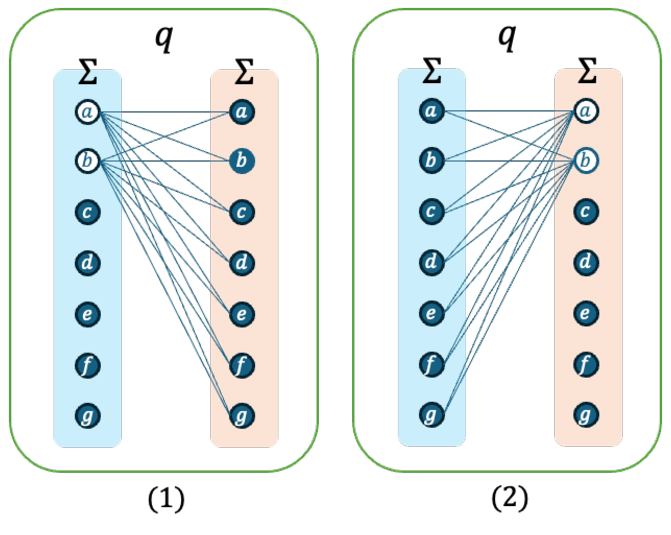
\includegraphics[scale=0.525]{figs/lem4bigraph.pdf}
    \caption{Let $\Sigma=\{a,b,c,d,e,f,g\}$ and $p,q \in \RPat$. We assume that the symbols in $\Sigma$ are mutually distinct.
    These figures (1) and (2) express two cases $D = \{ ay, by \}$ and $D = \{ ya, yb \}$, respectively.
    In these cases, if $p \{ x := r \} \preceq q$ for all $r \in D$, then $p \{ x := xy \} \preceq q$ holds.}\label{fig:lem4bigraph}
  \end{center}
\end{figure}